%----------------------------------------------------------------------------------------
%	DATA ACQUISITION AND PREPARATIONS
%----------------------------------------------------------------------------------------

\section{Data acquisition and organization}

The value and purpose of a study project does not only lie in the implementation and realization of a long-term scientific study - in our case, computer vision-based label prediction to improve an agricultural sorting machine. The intention is also to learn how to organize, schedule, and distribute tasks for a team over the period of one year. \\
 \\
To accomplish the objective of the project, a working structure had to be established. The project members had to learn each other's strengths and weaknesses to form a robust and efficient unit. Self-organization and team building became key to the success of the project. Thus, the secondary focus of the report lies on the management of the study group. \\
The process of team building and structuring is captured in the first half of this chapter. A timeline of the different working stages can be traced in a roadmap created at the start and updated at the end of the year. It reveals how well the team succeeded in predicting the duration of the various tasks. \\
Further, the communication between the members is addressed which includes regular meetings, agreements on different issues, or the working platforms that were used. Additionally, the teamwork is evaluated which comprises task distribution, the democratic working structure, and the structural integrity of the team. \\
After the organizational part of the project, the second half of this chapter is concerned with the collection of the data and the literature research. The sorting machine is described as well as the process of saving and retrieving the recorded images. It is followed by a summary of the literature which was thought to be relevant to our topic, regarding the visual detection of agricultural products or images with low variance with machine learning approaches. There was no specific paper, however, which could be used as a basis for our project. \\
\\
The first section of this chapter, 2.1 \textit{Roadmap of the project}, gives an overview of the time management of the study group. It is followed by the chapter 2.2 \textit{Organization of the study group}, in which communication and teamwork are assessed. In 2.3 \textit{Data collection}, the acquisition of the data from the sorting machine is described in more detail. The last section, 2.4 \textit{Literature research}, presents the retrieved literature concerning the issue of asparagus classification and agricultural product classification with machine learning based approaches.



\subsection{Roadmap of the project}

At the beginning of the project, a roadmap was created to structure the year into different working stages as well as to have an overview of the tasks and problems that needed to be addressed. Near the end of the year, this map was evaluated and updated to mirror the actual time spent at each project stage and to check how accurately the project had been planned from the start. If there were great discrepancies between estimation and reality, the map helped to acknowledge the wrong judgement of time and which working stages had taken longer than others. \\
\\
The following timetables in Figure~\ref{fig:Timetable} give a broad outline of the major stages of the project. In the left figure, it was estimated how much time for a specific phase is needed, whereas in the right figure the time spent for the stage is given. Both figures are structured to display the year in a circle, starting in April of 2019, and running clockwise through the year until April 2020. The months are represented by the inner circle while the outer circle marks the different working stages. \\
The project comprised four to five major stages. The following stage descriptions are shortened for the purpose of simplicity. A more detailed representation of the single tasks attributed to each stage can be found in the ensuing roadmaps in Fig.~\ref{fig:RoadmapPlanned} and Fig.~\ref{fig:RoadmapActual}. The project started with the Data Collection and the Organization of the study project. During the first stage, the images were recorded with the sorting machine, while the major planning and research for the project took place. In the second phase, most of the Preprocessing happened, that is, preparing and labelling the image data. This phase is split into two phases for the right figure displaying the actual time, ‘Preprocessing’ and ‘Labelling’. The classification stage includes the time spent on the machine learning approaches which were implemented and trained on the asparagus data. In the last stage, the approaches were evaluated and their results were compared. It is noteworthy that the different stages overlapped to a certain degree, because minor tasks of a previous stage were still in progress while tasks from the subsequent stage had already started. For the purpose of this figure the start and end time is displayed as a hard boundary. \\
\\

\begin{figure}[h]
	\centering
	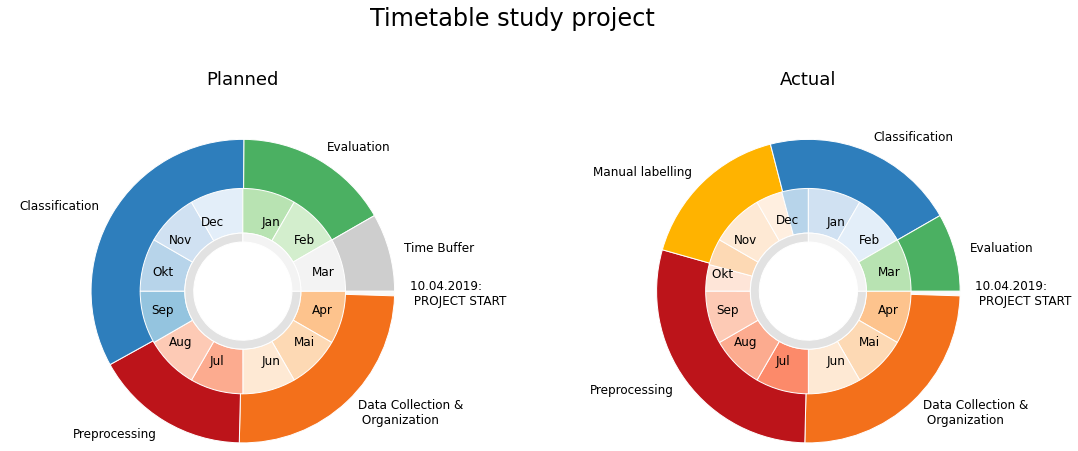
\includegraphics[scale=0.4]{Figures/chapter02/fig_timetable}
	\decoRule
	\caption[Timetable of the project]{On the left side is a timetable with the estimated time of the study project during the year from April 2019 to April 2020. To the right, the timetable displays how the time was spent.}
	\label{fig:Timetable}
\end{figure}

When comparing both figures, some distinctions can be recognized. The figure to the left shows that - while it was noted that the Preprocessing step of labelling the data would take some time - it was not estimated to take longer than until the end of August. Compared to the Preprocessing step in the right figure, it is observed that the phase continued until October. Furthermore, the time for labelling a sufficient amount of images was underestimated. In the right figure, the labelling process received its own stage to highlight the fact that it demanded much more effort and time compared to the initial estimation.
This exchange required that the time buffer and parts of the time calculated for the later stages of classification and evaluation had to compensate for the time loss.
The time difference can best be seen when comparing the respective colours (that is, the brighter colours of red, orange and yellow to the darker colours of blue and green). While the main focus of this project was supposed to be the application of different machine learning techniques to classify the data, the data generation and preprocessing posed to be the most time-consuming stages. \\
As a result, both timetables differ in that the year was more optimistically planned than realized. A major factor was the lack of experience of the participants concerning not only the conduction of a larger project with many co-workers but also the general implementation of the preprocessing stage for machine learning classification. Another factor influencing the shifted timeline was the working structure of the team. It was re-evaluated during October to better fit the needs of the group members and avoid distributing so-called ‘bottleneck’ tasks (that is, tasks that are decisive for the continuation of the next steps) to single members only. All in all, a valuable lesson learned during the project was to not underestimate a preprocessing phase. \\

\begin{figure}[h]
	\centering
	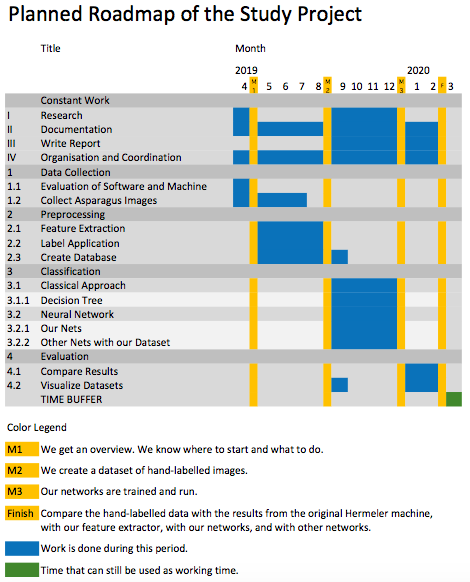
\includegraphics[scale=0.5]{Figures/chapter02/roadmap_planned}
	\decoRule
	\caption[Planned Roadmap]{The figure shows the planned roadmap of the study project. It reveals how the time needed for each task was estimated in the beginning of the project.}
	\label{fig:RoadmapPlanned}
\end{figure}

\begin{figure}[h]
	\centering
	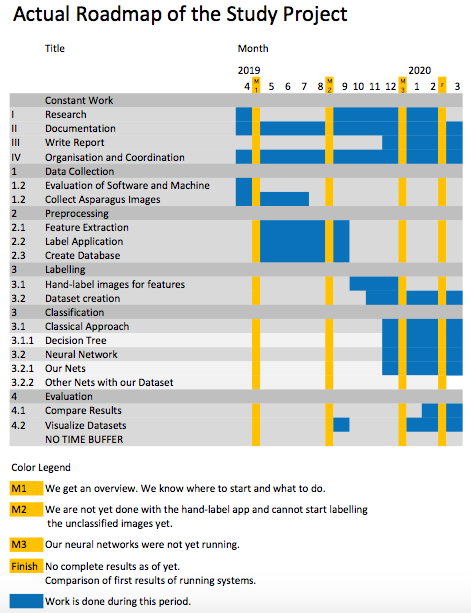
\includegraphics[scale=0.5]{Figures/chapter02/roadmap_actual}
	\decoRule
	\caption[Actual Roadmap]{A roadmap that shows how the time was spent.}
	\label{fig:RoadmapActual}
\end{figure}
\\
In Figure~\ref{fig:RoadmapPlanned} and Figure~\ref{fig:RoadmapActual}, the stage specific tasks can be seen in more detail. Again, both figures display the estimated time and the actual time, respectively. The headlines serve as the division into the major stages except for the first heading, ‘Constant Work’, which shows the tasks that demanded continuous attention and effort throughout the year. The duration of tasks is represented in blue, while the yellow lines mark milestones that are explained in their legends. \\
\\
Comparing both roadmaps, the shift of focus is seen more clearly and can be associated with the duration of single tasks. Especially the prominent drift of the classification stage mirrors the fact that the time estimation is worth improving. The roadmap helped to better assess the time needed for task completion.
In the following chapter, the management of the work distribution and the communication are taken into focus.


\subsection{Organisation of the study group}

In this chapter, we will describe how we have organized ourselves to work together on the project. For this we will elaborate on the tools we used for communication and organization as well as on the structure of our group work and our teamwork in general.


\subsubsection{Communication}

Our main way of communication were frequent meetings in which we discussed our process work period and distributed tasks for the next one. In addition to those meetings, we used different platforms, which worked with varying degrees of success. After a presentation about possible strategies of cooperation, we initially decided to use Asana, GitHub and Telegram to facilitate the communication outside of our meetings. The different means of communication will be described and evaluated in the following abstract. \\
\\
Regular meetings have been the most helpful in organizing our project. During the meetings, which usually lingered for one or two hours, there was a discussion leader and a protocol writer. The protocols were saved for review in our GitHub project. The meetings were characterized by long discussions about the best approach for the following steps and the possibilities to tackle the next challenge. Our supervisors were almost always present at the meetings, they brought in their expertise and gave us the opportunity to ask concrete questions. During the first half of the project, tasks were always distributed at the end of each meeting and in the next meeting the progress of the work was discussed. The communication was changed in the second half of the project,  where we started to use a schedule that described the different tasks and deadlines in detail, and to gather for co-working. The organizational meetings were continued and used to discuss the current status with Ulf and Axel. Everyone reported about his area of responsibility. This helped us to spend less time discussing and debating and more time working on our tasks. \\
Telegram is a cloud-based instant messaging service for the use on smartphones, tablets and computers. Since the first meeting, we had a constant conversation in a group chat on Telegram, in which we arranged us for the weekly meetings, planned handovers of keys/transponders for the room or informed each other about the status of the project. The group chat also created space for mutual motivation when needed. The majority of important information was exchanged via telegram. \\
Asana is used to distribute tasks and to communicate projects successfully. Many integrations of other applications, such as Slack, can help to achieve this. We used a board view where we listed tasks in different sections. But this function alone did not help us much in our project. The tasks were easier to distribute in direct consultation at physical meetings and demonstrated or discussed after completion. So it happened that asana was not used enough to be helpful. If we had relied on communication with Slack or other agreed services or applications, it might have made more sense, but asana alone was proven to be inefficient in our use case. \\
GitHub is a web-based popular plattform using a version control system using Git that helps developers store and manage their code, and track and control changes to their project. During the project, we learned how to use it. Initially, a presentation was given by Katharina on how to use Git, because there are a few rules to follow to keep it straightforward. Git allowed us to work from anywhere, which was very helpful for us. We also automatically created a documentation with Sphinx. This means that by using the GitHub project in the right style, the protocols, the work schedules, the manuals, and our code comments are automatically described in our documentation (\url{https://asparagus.readthedocs.io/en/latest/ }).


\subsubsection{Teamwork}

This subchapter outlines the team forming, the team members and the cooperation in our study project. It starts by introducing the team members and their previous experiences. This is followed by a description of the practical aspects of teamwork, the work structure, and the distribution of project-relevant tasks. \\
\\
First, the team members and their respective backgrounds are illustrated before delving into further work-related task distributions.
The project was an initiative of one of the students and, hence, a large part of the project members are friends that were inspired by her ideas. Other students joined the project after its public announcement to complete the team. Thus, the group consisted of members with varying degrees of knowledge about each other, which had an influence on the dynamics of the teamwork. The team was initially made up by Malin Spaniol, Maren Born, Katharina Groß, Josefine Zerbe, Michael Gerstenberger, Richard Ruppel, Sophia Schulze-Weddige, Luana Vaduva, Thomas Klein and Subir Das. None of the members had yet worked together as such on a project of this scope. During the course of the project, three members left the team for various reasons. Thomas left in July due to a change in his study program. This was an unfortunate occurrence because he posed a valuable source of knowledge in the field of computer vision. Further, Luana and Subir left in October to pursue different study projects. \\
\\
By the start of the project, all except two of the members were in their master’s degree in Cognitive Science at the University of Osnabrück. The members brought a wide variety of backgrounds into the team through different bachelor programs or different majors in the broader field of cognitive science.
In the beginning of the project, the team members had little to no experience in the application of computer vision or neural networks. The motivation of most students was to pursue new and interesting tasks in these fields. Four students had a theoretical background in computer vision, six students had gained some experience with neural networks through the course ‘ANN with Tensorflow’, taught at the University of Osnabrück, while some had also taken machine learning classes during their study program. None of the members had prior knowledge about project management or task organization on a broader level. Git was previously only used by three students so far, but none of them were experts on its usage. Further, no participant had any experience with the Grid system of the IKW, not to mention running jobs on different machines.
Thus, the project started with 10 members, where each of the participants brought a different level of experience in the most relevant fields of machine learning, that is computer vision and neural networks, into the team. \\
\\
After introducing the team members and their backgrounds, this section continues with elaborating the structural organization of the team and the work distribution.
As none of the members had any previous experience with team formation, in the beginning, the team lacked some structure and a clear distribution of single roles inside the team. One reason for this was the harmonious atmosphere between the single members. Many of the team members had a friendly relationship already from the start of the project. Also, further tasks at the beginning, like the trips to the asparagus farm, strengthened the team spirit and the social interactions positively. So we started with a very dynamic structuring of tasks by making every decision democratically. As described in more detail in the next chapter, we first used the joint meetings to distribute the tasks. As an example, we had to prepare a schedule for organizing the data collection and already started with preprocessing tasks. These two main activities were mostly done in smaller teams of two to three people. Rather few tasks were done alone. In our meetings, we often formulated possible next tasks, even for the distant future, but as the project progressed we did not assign them to a specific person or working group. \\
In August, we restructured our own organization. On the one hand, this was due to the fact that the tasks changed and thus a new structure was more appropriate. On the other hand, also the strength of the individual team members were a reason for the restructuring. Some team members had less programming experience than others and therefore had difficulties realizing certain tasks at the same time and with the same precision than others. Even if they had good ideas in terms of concept, it was not possible for them to implement these ideas quickly enough so that they could be included into the project. Nevertheless, there was still the possibility to grow in his new assignments. In addition, the democratical self-organization and difference in programming expertise led to a distortion in the time management of the group and some tasks were not finished in time. To integrate more of the strengths that the single team members brought and to tackle the issue of time management, it was decided to write a roadmap that distributed the work more appropriately, gave an overview of the tasks that still had to be done and how much time was left to do them. \\
Further, common working hours on campus were introduced as well as a division of responsibilities which were work-related and related to the supervision of tasks. The common working hours ensured that questions and decisions that arose could be discussed directly. This was especially helpful when different tasks overlapped and required communication and agreement.
The supervision of the work was divided into manager roles, which means that the work was split into different main fields where each member was responsible for managing their assigned area, distributing tasks and keeping an overview of the relevant work inside their working field. Furthermore, one knew who to turn to for questions and when in need of discussion or feedback. The meetings became more effective due to the new structure, and there was less discussion concerning task distribution. As we distributed roles, we were also more responsive to the strengths and weaknesses of the group members. Therefore one can say that the team structure and distribution of work changed over the course of the project. The strengths of single members were used more efficiently and the supervision of working areas led to a more structured supervision and manageable task distribution. \\
\\
In the course of the project and to sum up the focus of this chapter, namely the organisation of our study group, it can be said that we had a harmonious team with two different working structures. The first one cultivated at the start of the project and the other one at the end of the project, respectively, which happened due to the tasks amount and the optimisation of our teamwork. We have all learned that teamwork is not a trivial issue, even for members who already know each other well.


\subsection{Data collection}

In this section, the process of recording and assembling the data is described, together with information about the asparagus sorting machine ‘Autoselect’.
For the data collection, the project group had to drive to the asparagus farm “Gut Holsterfeld” at Rheine. First expectations to receive only labelled data were disappointed. The farmer was not able to provide the amount of labelled data that was needed for the project. As the asparagus season was about to start, the first two months of the project were mainly dedicated to data collection. \\
 \\
First, the asparagus sorting machine at Gut Holsterfeld is described before reporting about the process of labelled and unlabelled data collection.
The machine ‘Autoselect ATS II’ (2003) is designed for sorting white asparagus and green asparagus~\citep{autoselectanleitung}. The sorting is based on the parameters width, length, shape, curvature, rust, and colour. A total of 30 criteria for classifying an asparagus spear are used to describe these parameters. The calculation of the single features is based on a classical analytical approach. For example, the feature colour is composed of 8 sub-parameters. Each spear is reviewed at different areas (the head of the asparagus, the area below the head, and the stem, respectively) and judged for its hue in percentage. The values are compared and, according to a threshold, the spear is sorted into a colour category. For all parameters, there is a minimal threshold and a maximal threshold. As another example, the parameter width is calculated at three points at the asparagus (top, middle, and bottom part). From these three values, an average value is calculated that decides in which category the asparagus is sorted. If an asparagus exceeds the maximal threshold, it is not recognized and cannot be sorted accordingly. Thus, all parameters have to have an upper and a lower threshold, including parameters like shape, curvature, and colour. When evaluating which thresholds to choose, it is recommended to check that most asparagus spears tend to be in between the average value and the maximal threshold, with a larger tendency to accumulate around the average value. All parameters can be freely chosen by the farmer and can this way be fitted to the needs of the respective asparagus farm. \\
According to the manual, the number of classifications (quality classes) is selectable but it is based on the number of output trays available to the machine. The machine Autoselect at “Gut Holsterfeld” has 16 trays. The program of the Autoselect processes the sorting parameters from the best class to the worst class. The user can define the order of parameters. The manufacturer suggests to first sort for length and width, then sort for colours parameters, and analyze the shape parameters last. 


\begin{figure}
    \centering
    \subfloat[]{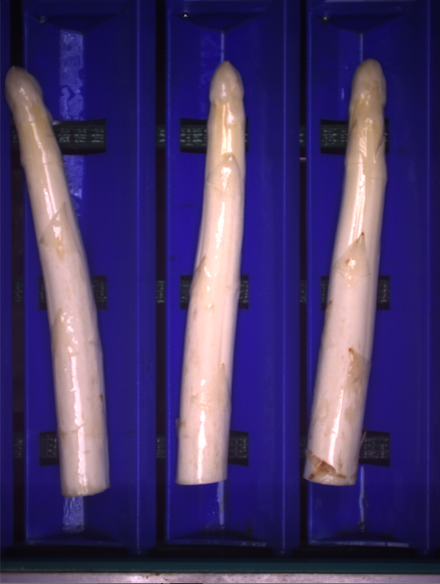
\includegraphics[width=4cm]{Figures/chapter02/anna_a}}
    \qquad
    \subfloat[]{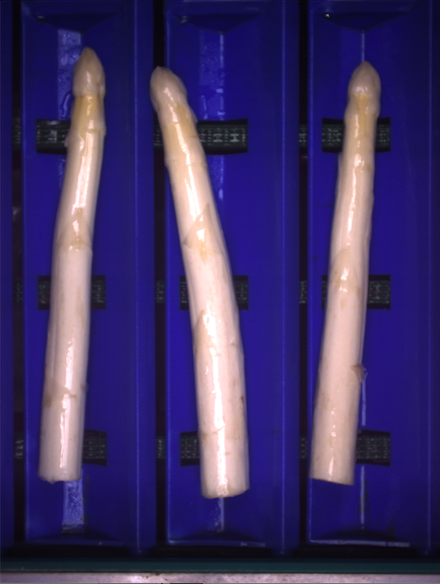
\includegraphics[width=4cm]{Figures/chapter02/anna_b}}
    \qquad
    \subfloat[ ]{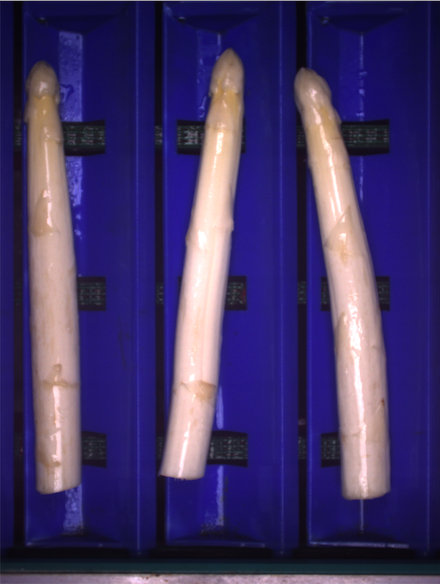
\includegraphics[width=4cm]{Figures/chapter02/anna_c}}
    \caption[Example of asparagus images]{Example pictures of the quality class I A Anna. In picture (A), the asparagus spear is to the right, in (B), it is in the middle, and in (C) it is to the left.}
    \label{fig:ExampleImagesAnna}
\end{figure}

The sorting process of the software is performed in a certain order according to the quality, with asparagus of the best quality classes being collected in the first trays. Before the first use of the machine, all parameters are selected after the first sort has run through the machine. Then, the user can fit the thresholds accordingly.
The asparagus is arranged on a conveyor belt that runs it through the recording section of the machine. Here, a camera takes three pictures per asparagus as seen in Figure~\ref{fig:ExampleImagesAnna}. Small wheels on the conveyor belt rotate the asparagus in the meantime so that it can be photographed from several positions. In the best case, on each image a different side of the asparagus is recorded. The conveyor belt transports the spear further and it is sorted into a tray depending on the chosen quality class by the machine. \\
The accuracy of the sorting machine is described to be as good as 90\% best case by the manufacturer, while the farm reported it to be best around 70\%, with re-sorting being necessary by professional sorters. Especially categories like Blume or Hohle were considered to be inconsistent - if no better than chance - by both, manufacturer and farmer. Further information could not be given on the software of the machine. A meeting with a representative of the engineering company HMF that manufactured the sorting machine was arranged (\url=www.hmf-hermeler.de). Unfortunately, the software itself was not available to HMF as it was produced by another specialized company. During the meeting, it was discovered that the quality of the camera might be highly relevant for the accuracy of the sorting machine. Luminance and resolution are decisive for the quality of the image. Thus, technical restrictions for the sorting process had to be expected, also for our idea of implementing techniques based on machine learning.\\
\\
In the following it is described how the image data was collected. It was possible to save images with the Autoselect, however, the storage space on the machine was very limited. Whenever its C storage was full, the machine stopped and the sorting process was interrupted. This caused not only problems to the storing of images but also to the asparagus farm who had to rely on the machine for the sorting. Further, the selection of images to be saved was restricted to only 1000 images. Any number chosen above 1000 led to the machine saving every image until the storage was full and the machine stopped (i.e., when instructing to save 1001 images, the machine would ignore the number and save images up to its breaking point). \\
One solution to the image selection problem was the installation of the Teamviewer software on the machine. For this, the machine had first to be connected to the internet at the farm, where only restricted internet access was possible. After the Teamviewer installation, the process of image collection could be started remotely. This work was very ineffective and time-consuming because the process had to be restarted every 1000th picture. Further, there was still the problem of limited storage. The data could not be directly transmitted to another computer because the internet connection at the farm was not stable enough. Therefore, an external storage was connected to the machine. Further, automatic transfer of the images to the external harddrive was not possible but the images had to be transferred manually, again via Teamviewer. A solution to the problem was the installation of an automatic file moving service, for which the requirements are described below. \\
A program was needed that transfers the images to a new saving destination to resolve the problem of limited storage and manual transfer. It had to run in the background and should not disturb the workflow during the sorting process. The operating system on which the sorting machine runs is Windows. After some internet research on background processes and programs, the decision was made to use a service, that is, a system process running independently of any program. As Windows was used, the development was done with the DOTNET framework in the programming language C#. The package provided is called Topshelf (\url{https://github.com/Topshelf/Topshelf}). Topshelf is a service hosting framework for building Windows services using .NET (\url{https://docs.microsoft.com/en-us/dotnet/framework/get-started/overview}). Like this, it is possible to develop a console application in the development phase, compile it as a service, and install it later via the console. Previously, it was not possible to debug services. The function of the service is based on the FileSystemWatcher object (\url{https://docs.microsoft.com/en-us/dotnet/api/system.io.filesystemwatcher?view=netframework-4.8}) from the System.IO namespace. In the main program, a list of files in the source folder is kept. Files that are older than one hour are moved to the target folder on the external drive. The selected files are moved by a function that is called, when an event is triggered. The event is triggered by the FileSystemWatcher after subscribing to different flags. After a short time the service was adjusted. An hourly waiting time was then introduced via Teamviewer sessions because the program of the sorting machine itself still accessed the image number indefinitely and therefore image collection had to be started every 1000th image. \\
\\
Another issue concerning the storage space for collecting the image data was that the external harddrive ran full after 2 to 3 sorting days. The project members split in groups of 2 and exchanged the harddrive two times a week. The collected images were then transferred to storage capacities of the university with the support of the project’s supervisors. \\
A last problem that had to be considered was that of unlabelled data. Before the project had started, the farm had not collected any labelled data and we could not rely on the labels that the machine attributed to each asparagus. A solution was to send the already sorted asparagus a second time through the machine. Like this it was assumed that we can not only receive labelled data but also acquire the parameters calculated by the machine. Unfortunately, it was not possible to extract the parameters from the machine. Another issue was posed by the fact that a second sorting is not good for the quality of the asparagus spears. Running them through the machine damaged some spears or led to the exclusion of certain spears from a good quality class into a worse quality class. Further, at least one project member had to be involved in the re-sorting and, thus, had to be present at the farm. The sessions of exchanging the external harddrive and collecting labelled image data were then combined. \\
\\
An example image of the received data can be seen in Figure~\ref{fig:ExampleImagesAnna}. There are three pictures per spear. The image resolution is around 1040$3\times4$ 1376 pixel per image, with an RGB colour space. \\
All in all, the number of collected, unlabelled data is above XX images, thus, above XX asparagus spears. Of the labelled data, we collected 1005 images with the label I A Anna,  908 images for I A Bona, 513 images of I A Clara, 936 images of I A Krumme, 1514 images of I A Violett, 1051 images of II A, 1468 images of II B, 1169 images of Rost, 749 images of Dicke, 775 images of Hohle, 1717 images of Blume, 1157 images of Suppe, and at least 309 labelled as Bruch. The image number does not represent the number of different asparagus spears, as each spear is represented by three distinct images. \\

\begin{figure}
    \centering
    \subfloat[]{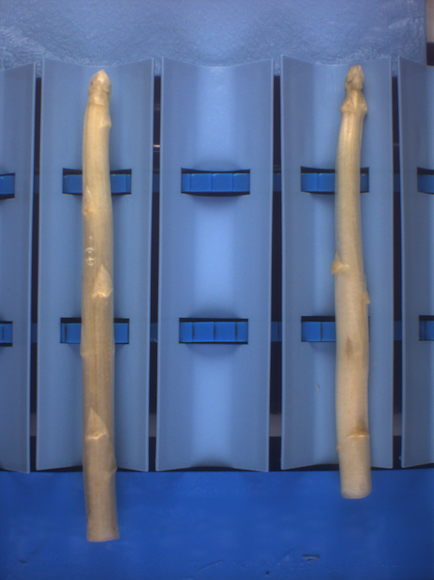
\includegraphics[width=3cm]{Figures/chapter02/querdel_a}}
    \qquad
    \subfloat[]{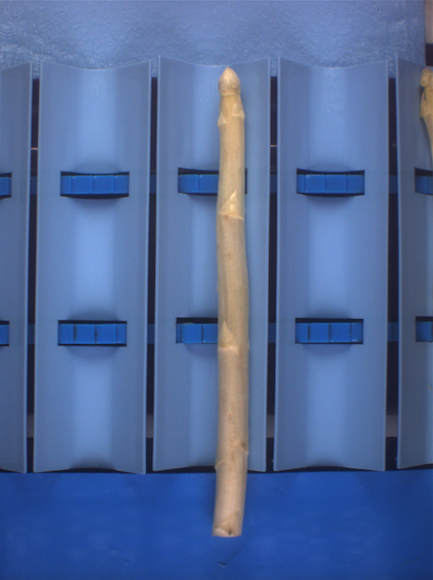
\includegraphics[width=3cm]{Figures/chapter02/querdel_b}}
    \qquad
    \subfloat[ ]{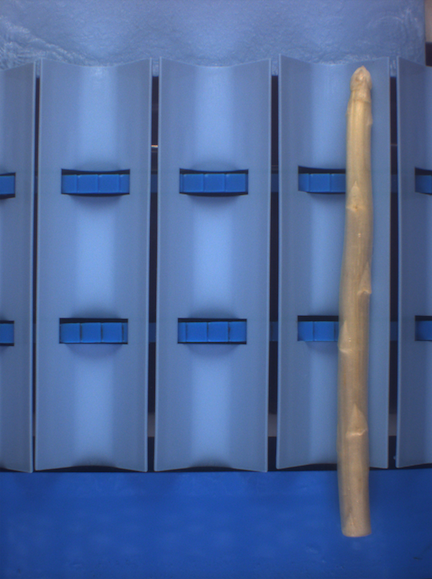
\includegraphics[width=3cm]{Figures/chapter02/querdel_c}}
    \qquad
    \subfloat[ ]{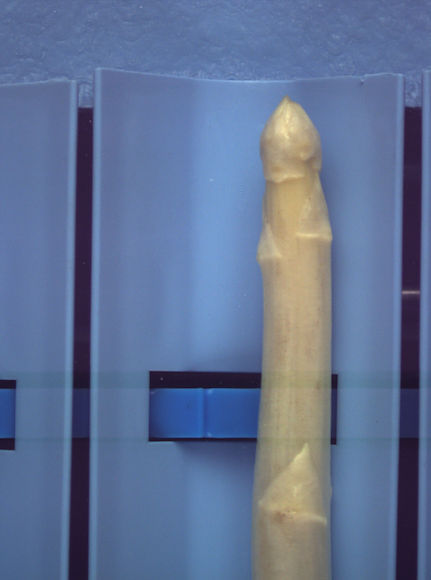
\includegraphics[width=3cm]{Figures/chapter02/querdel_d}}
    \caption[Example of asparagus images of Querdel's Hof]{Example pictures of the asparagus farm "Querdel's Hof". In picture (A), the asparagus spear is to the right, in (B), it is in the middle, and in (C) it is to the left. A fourth picture (D) is taken with a second camera with focus on the head}.
    \label{fig:ExampleImagesQuerdel}
\end{figure}

Most image data, that is XX image samples, was received from the asparagus farm “Gut Holsterfeld”. Additionally, a few images could be recorded at another asparagus farm, “Querdel’s Hof”, in Emsbüren (\url{https://www.querdel.de/}). The farm sorts the asparagus with an updated version of the Autoselect machine at “Gut Holsterfeld”, that is, it uses the same software but other hardware. The difference of both machines is purely in hardware, in particular the resolution of the camera was improved and a second camera was installed that focuses on the head region of the asparagus. At “Querdel’s Hof”, we collected 20616 images in total, 76 from the class ‘normal’, 152 from the class ‘violet/flower’, and 20388 unlabelled images. Of the data, an asparagus spear is represented by four images: three images show the same asparagus from different perspectives and a fourth image depicting solely the head region. An example image can be seen in Figure~\ref{fig:ExampleImagesQuerdel}. No internet connection could be established to the farm, thus, no further images were collected. Moreover, the class labels of asparagus spears as well as the data format of the images from “Querdel’s Hof” are different to the data from the farm “Gut Holsterfeld”, due to the additional head image. Therefore a combination of both data sets was not convenient. A further reason for no more collected data at the second farm was that the objective behind the study project was primarily the implementation of new software regarding the machine type Autoselect at the farm “Gut Holsterfeld”. \\
\\
To summarize this section, of the XX images collected in total, mostly unlabelled data was collected from the sorting machine Autoselect at the asparagus farm Gut Holsterfeld. Of the labelled data, each class of asparagus is represented with at least XX images (corresponding to XX spears).


\subsection{Literature research}

In the classification of food products, there seems to be a large field of different possibilities to apply classical machine learning, and also artificial neural network approaches for classification tasks on image data~\citep{bhargava2018fruits} ~\citep{brosnan2002inspection}. \\
Although, none of the papers that were found could be used as a blueprint to the asparagus classification project, some of them helped to get a better idea of how to proceed with the project, how to give structure to our preprocessing phase, or evaluate the machine learning methods that were already used on other food classification tasks~\citep{mery2013automated} ~\citep{bhargava2018fruits}. For example, some of the literature was concerned with the evaluation of food products but not with differentiating between as many classes as 13~\citep{diaz2004comparison} ~\citep{kilicc2007classification}. Often, the variance in the food products used was either too high~\citep{zhang2012classification} or too low~\citep{kilicc2007classification} ~\citep{al2011dates}.  One paper even evaluates the sorting of asparagus, however, only on a small dataset with three categories of green asparagus~\citep{donis2016classification}. Further papers discovered on food classification were not detailed enough in their approaches and, thus, not sharing any information needed for our task~\citep{pedreschi2016grading}. Other papers were mainly interested in the implementation of a certain toolbox~\citep{mery2013automated}. \\
Besides the search for food related classification tasks, further research was done for evaluating the use of a semi-supervised learning approach. As the available data was only sparsely labelled an idea was to engage with approaches relying on semi-supervised learning~\citep{olivier2006semi}~\citep{zhu05survey}. Details about the regarding literature can be found in the respective chapter 4.3. There, a semi-supervised approach is used in the implementation of a variational aoutencoder. In regards to deep learning-based approaches, classical neural networks - such as AlexNet, VGG16/VGG19, GoogleNet, Capsule Networks,  DenseNet, ResNet or Network in Network (NIN) - were assessed and presented for better understanding of the range of possible pre-trained networks and ideas for network structures~\citep{alexnet2012original} ~\citep{vgg2014original} ~\citep{googlenet2015original} ~\citep{capsulenet2017original} ~\citep{densenet2017original} ~\citep{resnet2016original} ~\citep{lin2013network}. Also, classical computer vision approaches were considered, like multiclass support-vector-machines~\citep{prakash2012multi}. \\
Another subject of extensive research posed the evaluation of our manual labelling of the unlabelled data (see chapter 3.4). For this, different methods were compared and an agreement measure was chosen~\citep{mchugh2012interrater}. Especially for later task distribution during the project year, literature research was mainly done in smaller groups of one or two and only discussed with the group if it was relevant to the team. \\
\\
In conclusion, the time given for further research in a group was efficiently used. The design of a structured framework for collecting research literature could not be established. Except for the first few weeks into the project, there was no unified literature research during the project. Rather, every member consulted literature on their own for the specific tasks and problems everyone had to face. Like this, most of the papers that were used as inspirations or basis to certain tasks and approaches can be found throughout the report.

